\documentclass[table, usenames,dvipsnames,svgnames]{beamer}
\usetheme{CambridgeUS} 
\usecolortheme{default}

\RequirePackage{xeCJK}
\RequirePackage{fontspec}


\setCJKmainfont{WenQuanYi Micro Hei}

\title[Approximate Counting and Sampling]{\Large{Approximate Counting and Sampling}\\\vspace{2mm}\normalsize{Brief Introduction with a Few Examples}}
\author[LIU Shuang]{劉爽}
\institute[SJTU ZY ACM 2012]{上海交通大學致遠學院2012級ACM班}
\date[2013.11.29]{2013.11.29}

\begin{document}

\begin{frame}
    \titlepage
\end{frame}

\section{Counting}

\subsection{Definition}
\begin{frame}
    \frametitle{FPRAS}
    \pause
    \begin{definition}[($\epsilon$, $\delta$)-approximation]
        A randomized algorithm gives an ($\epsilon$, $\delta$)-approximation for the value $V$ if the output $X$ satisfies:
        $$
        Pr(|X - V|\leq \epsilon V) \geq 1 - \delta
        $$
    \end{definition}
    \pause
    \begin{definition}[FPRAS]
        A fully polynomial randomized approximation scheme (FPRAS) for a problem is a randomized algorithm for which, give an input X and any parameters $0 < \epsilon, \delta < 1$, the algorithm outputs an ($\epsilon$, $\delta$) approximation to $V(x)$ in $1/\epsilon$, $ln\delta^{-1}$ and the size of the input $n$.
    \end{definition}
\end{frame}

\begin{frame}
    \frametitle{Monte Carlo Method}
    \pause
    \begin{definition}[Monte Carlo Method]
        Use an efficient Process to generate a sequence of independent and identically distributed random samples with $\mathbb{E}[X_i] = V$. Get enough samples for an ($\epsilon$,$\delta$)-approximation for $V$.
    \end{definition}
\end{frame}

\begin{frame}
    \frametitle{Dart Throwing}
    \pause
    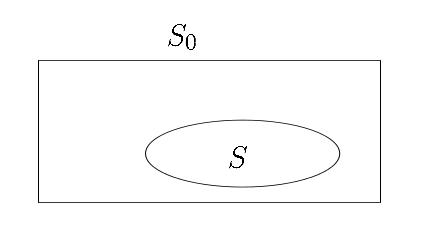
\includegraphics[height=30mm]{dart.jpg}
    \pause
    \begin{itemize}
        \item Suppose we want to estimate $|S|$, we find a set $S_0 \supseteq S$, the size of which $|S_0|$ is known, and it is easy to pick a (near) random member of $S_0$
            \pause
        \item To estimate $|S|$ we choose random points from $S_0$ and estimate $\frac{|S|}{|S_0|}$ by the proportion of samples that are in $S$.\pause
        \item How large should the ratio $\frac{|S|}{|S_0|}$ be?
    \end{itemize}
\end{frame}

\begin{frame}
    \frametitle{Dart Throwing}
    \pause
    \begin{itemize}
        \item We generate $M$ random variables $X_i$ and take $\mu = \frac{\sum{X_i}}{M}$ as our estimation \pause
        \item denote $V = |S|$ and $V_0 = |S_0|$, since $\mathbb{E}(X_i) = V$, we have $\mathbb{E}(\mu) = V$ \pause
        \item If we use Chebyshev inequality, we have
            $$
            \Pr(|\mu - V| \geq \epsilon V) \leq \frac{Var(X)}{M\epsilon ^ 2 V ^ 2} \leq \delta
            $$
            $$
            M \geq \frac{Var(X)}{V ^ 2}\frac{1}{\epsilon ^ 2 \delta}
            $$\pause
            \item we need $\frac{Var(X)}{V^2}$ to be $poly(n)$\pause
            \item Since $Var(X) \leq V_0^2$, We only need $\frac{V}{V_0} = \frac{1}{poly(n)}$ 
    \end{itemize}
\end{frame}

\begin{frame}
    \frametitle{Dart Throwing}
    \pause
    \begin{itemize}
        \item If we estimate $\frac{V}{V_0}$ instead and also suppose $X_i$ takes value from $\{0, 1\}$, we can use Chernoff bound, we have
            $$
            \Pr(|\mu - \frac{V}{V_0}| \geq \epsilon \frac{V}{V_0}) \leq 2e^{-\frac{\epsilon ^ 2 MV}{3V_0}} \leq \delta
            $$
            $$
            M \geq \frac{3ln\frac{2}{\delta}}{\epsilon ^ 2}\frac{V_0}{V}
            $$\pause
            we need $\frac{V}{V_0}$ to be $\frac{1}{poly(n)}$
    \end{itemize}
\end{frame}

\subsection{Example}

\begin{frame}
    \frametitle{\#DNF-SAT}
    \pause
    \begin{definition}[DNF]
        In boolean logic, a disjunctive normal form (DNF) is a standardization (or normalization) of a logical formula which is a disjunction of conjunctive clauses
        $$
        (A \wedge \neg B \wedge \neg C) \vee (\wedge D \wedge E \wedge F) \vee (\neg A \wedge F)
        $$
    \end{definition}
\end{frame}

\begin{frame}
    \frametitle{\#DNF-SAT}
    \pause
    \begin{itemize}
        \item Suppose there are $n$ variables and $k$ be the number of clauses\pause
        \item A first approach, choose $S_0$ be the all $2^n$ assignments. \pause
        \item $\frac{|S|}{2^n}$ should be $\frac{1}{poly(n)}$, but we don't know the size of $S$
    \end{itemize}
\end{frame}

\begin{frame}
    \frametitle{\#DNF-SAT}
    \pause
    \begin{itemize}
        \item A better approach, construct a matrix
            \\
            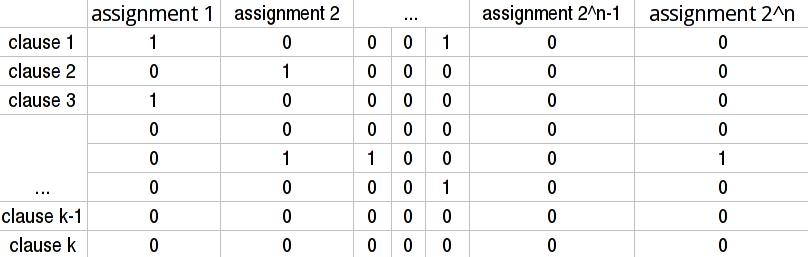
\includegraphics[height=30mm]{table.jpg}\pause
        \item $C_{ij} = 1$ if clause $i$ can be satisfied by assignment $j$, $0$ otherwise.\pause
        \item $S_0 = \{\text{number of ones in the matrix}\}$

            $S = \{\text{columns contain at least one}\}$
                
        \item In other words

            $S = \{\text{the uppermost one in each column}\}$
\end{itemize}
\end{frame}

\begin{frame}
    \frametitle{\#DNF-SAT}
    \pause
    \begin{itemize}
        \item First we show $\frac{|S|}{|S0|}$ is not too small
            $$
            \frac{|S|}{|S_0|} \geq \frac{1}{k}
            $$\pause
        \item Then we show elements in $S_0$ can be generated uniformly at random
    \end{itemize}
\end{frame}

\begin{frame}
    \frametitle{\#DNF-SAT}
    \pause
    \begin{itemize}
        \item Suppose there are $R_i$ ones in row $i$, then we have $R_i = 2^{n - d_i}$, where $d_i$ is the number of variables in the $i_{th}$ clause. Let $R = \sum R_i = |S_0|$.\pause
        \item We choose row $i$ with probability $\frac{R_i}{R}$, and then determine each of the variable not in clause $i$ uniformly at random, thus get the $2^{n - d_i}$ ones in column $i$ uniformly at random.\pause
        \item Finally, if the chosen one is the uppermost one in its column, we let $X_i$ be $1$, otherwise be $0$.
    \end{itemize}
\end{frame}

\begin{frame}
    \frametitle{\#DNF-SAT}
    \pause
    \begin{itemize}
        \item If we repeat $M$ times, our estimation thus is $\frac{\sum X_i}{M}|S_0|$ \pause
        \item Give $\epsilon$ and $\delta$, Let $M = \frac{3kln\frac{2}{\delta}}{\epsilon^2}$, this algorithm gives an ($\epsilon$, $\delta$)-approximation, thus is a FPRAS.
    \end{itemize}
\end{frame}


\section{Sampling}

\subsection{Definition}

\begin{frame}
    \frametitle{FPAUS}
    \pause
    \begin{definition}[Variation Distance]
        The variation distance between two probability distributions $\pi$ and $\pi'$ on a countable state space $S$ is given by 
        $$
        \|\pi - \pi'\| = \frac{1}{2}\sum_{x\in S}|\pi(x) - \pi'(x)|
        $$
    \end{definition}
    \pause
    \begin{definition}[FPAUS]
        An almost uniform sampler (AUS) is a randomized algorithm that takes as input of size $n$ and a tolerance $\delta$, and produces a random event $F \in \Omega(x)$, such that the probability distribution of $F$ is within variation distance $\delta$ of the desired distribution on $\Omega(x)$. A fully polynomial almost uniformly sampler is an AUS runs in poly-time in $n$ and $ln\delta ^{-1}$
    \end{definition}
\end{frame}

\begin{frame}
    \frametitle{Markov chain Monte Carlo Method}
    When the samples cannot be sampled "directly", we often use the following method
    \begin{definition}[MCMC]
        The Markov chain Monte Carlo (MCMC) Method runs as follows: Define an ergodic Markov Chain $\mathcal{M}$ with states the elements of the sample space, $\mathcal{M}$ must converge to the requered distribution fast enough (as a FPAUS). From any starting state and after a sufficient number of steps $r$ the distribution of $X_r$ will be close to the stationary distribution, and we use as almost independent samples $X_r, X_{2r}, X_{3r} \dots$
    \end{definition}
\end{frame}

\subsection{Example}

\begin{frame}
    \frametitle{K-Colouring}
    \pause 
    \begin{itemize}
        \item Let G = (V, E) be a graph of maximum degree $\Delta$. We want to uniformly at rondom sample proper k-colourings of G (use k colours to paint the vertices so that any adjacent vertex have different colours). Here we will assume that $k > 2\Delta$.
    \end{itemize}
\end{frame}

\begin{frame}
    \frametitle{K-Colouring}
    \pause
    \begin{lemma}
        For a finite space $\Omega$ and neighborhood structure $\{N(x) | x \in \Omega|\}$. Let $N = max_{x\in \Omega}|N(x)|$.Let $M \geq N$. If the following MC is irreducible, aperiodic then the stationary distribution is the uniform distribution.
        $$
        P_{x,y} = \begin{cases} \frac{1}{M} &\mbox{if } x \neq y \mbox{ and } y \in N(x), \\
    0 &\mbox{if } x \neq y \mbox{ and } y \not\in N(x), \\
    1 - \frac{N(x)}{M} &\mbox{if } x = y, \end{cases}
        $$
    \end{lemma}
\end{frame}

\begin{frame}
    \frametitle{K-Colouring}
    \pause 
    \begin{itemize}
        \item Let's define a Markov chain on $\Omega(k, G)$.\pause
        \item \textbf{Step 0} $X_0$ is any k-colouring of $G$
        \item \textbf{Step t} Choose v uniformly at random from V and i uniformly at random from 1 to k, try to re-colour v in $X_{t-1}$ with colour i. If succeed, $X_t$ should be the re-coloured graph, otherwise, $X_{t}=X_{t-1}$.\pause
        \item This chain obviously satisfies of the requirements of the previous lemma.
    \end{itemize}
\end{frame}

\begin{frame}
    \frametitle{K-Colouring}
    \pause 
    \begin{definition}[Mixing Time]
        Let $p^t_x$ be the distribution of the state of a Markov Chain starting at x after t steps and $\pi$ be the desired stationary distribution. We define
        $$
        \Delta_X(t)=\|p_x^t-\pi\|
        $$
        We define $\tau_{X}(\epsilon)=min\{t|\Delta_{X}(t)\leq \epsilon\}$ and the mixing time $\tau(\epsilon)=max_{X\in S}\tau_X(\epsilon)$.

        A chain is called rapidly mixing if $\tau(\epsilon)$ is polynomial in $\frac{1}{\epsilon}$ and the size of the problem $n$.
    \end{definition}
    Jerrum showed that if $k > 2\Delta(G)$ then the mixing time of the chain defined previously is $O(kn\log n)$
\end{frame}

\section{Relationship}

\subsection{Sampling to counting}

\begin{frame}
    \frametitle{From good sampling to approximate counting}
    \pause 
    Now we want to estimate the number of k-colourings of a graph.
    \begin{theorem}
        Suppose we have a AUS for the k-colouring of a graph, which works for graphs $G$ with maximum degree bounded by $\Delta$ and suppose that the sampler has time complexity $T(n,\delta)$. Then we may construct an FPRAS for the number of k-colouring of a graph, with degree bound $\Delta$ and time complexity 
        $$
        O(\frac{m^2}{\epsilon ^2}T(n, \frac{\epsilon}{6m}))
        $$
        where $m$ is the number of edges in $G$ and $\epsilon$ the specified error bound.
    \end{theorem}
\end{frame}

\begin{frame}
    \frametitle{From good sampling to approximate counting}
    \pause 
    \begin{proof}[Proof outline]
        Let $\Omega(k, G)$ denote the set of proper k-colourings of G. Let $E = \{e_1, e_2, \dots, e_m\}$ and let $G_i = (V, \{e_1, e_2, \dots, e_i\})$. Then
        $$
        |\Omega(k, G)|=|\Omega(k, G_0)|\prod^m_{i=1}\frac{|\Omega(k, G_i)|}{|\Omega(k, G_{i-1}|}
        $$
        Since $|\Omega(k, G_0)|=k^{|V|}$, we only need to estimate the ratios
        $$
        \rho_i=\frac{|\Omega(k, G_i)|}{|\Omega(k, G_{i-1})|}
        $$
        Then we can use MCMC to choose near random members of $\Omega(k, G_{i-1})$ and seeing what proportion are also in $\Omega(k, G_i)$. Since $k > 2\Delta$, $\rho_i > \frac{1}{2}$, which prevents the failure of the sampling.      
    \end{proof}
\end{frame}

\subsection{Counting to sampling}

\begin{frame}
    \frametitle{From approximate counting to good sampling}
    Let's take the number of independent sets as our example (which is quite similar to k-colouring)
    \pause 
    \begin{theorem}
        Suppose we have an FPRAS $APPROXCOUNT(G, \epsilon, \delta)$ for the number of independent sets of a graph $G = (V, E)$ and suppose that $APPROXCOUNT(G, \epsilon, \delta)$ has time complexity $T(n, \epsilon, \delta)$. Then we can construct a AUS $U_{GEN}$ which has expectd time complexity 
        $$
        O(T(n, O(\frac{1}{n}), O(\frac{\delta}{n})))
        $$
    \end{theorem}
\end{frame}

\begin{frame}
    \frametitle{From approximate counting to good sampling}
    \pause 
    \begin{proof}[Proof Idea]
        Construct an algorithm as follows:
        There is a function called $U_{GENX}$, we call it repeatly untill we get an sample.
        The function $U_{GENX}$ has an argument $\phi$ roughly means the probablity of failure.

        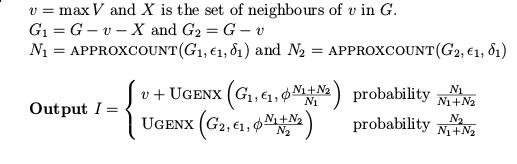
\includegraphics[height=35mm]{prog.jpg}
    \end{proof}
\end{frame}

\section{Thank you}

\begin{frame}
    \frametitle{Thank You}
\end{frame}

\end{document}
